% !Mode:: "TeX:UTF-8"
%%==========================
%% chapter01.tex for SJTU Master Thesis
%% based on CASthesis
%% modified by wei.jianwen@gmail.com
%% version: 0.3a
%% Encoding: UTF-8
%% last update: Dec 5th, 2010
%%==================================================

%\bibliographystyle{sjtu2} %[此处用于每章都生产参考文献]
\chapter{背景知识}
\label{chap:back}
在本章中,我们会介绍一些我们工作中涉及到的背景知识,了解这些背景知识,有助于更好的了解本文要解决的问题,以及本文的贡献所在。
主要会分为四方面内容去介绍,一是图模型,这是机器学习中非常重要的一个模型,可以很好的表示变量之间的关系,从而利用图结构模型去解决问题;
二是图画式结构,这是计算机视觉领域中提出来的,主要是针对弹簧模型中的预测算法会使用到。
三是结构式学习,这是很多机器学习问题都需要使用的算法,因为很多问题的结构都是一个结构化的输出,所以结构式学习在解决这方面问题上扮演了很重要的角色。
最后一个是形变部位模型,这是人体姿势识别领域最经典和最成功的模型,它将人体躯干部位作为隐变量,取得了很好的预测效果。
很多后人的工作,都是基于形变部位模型去做各种变形和改进。
我们的工作也不例外,基于形变部位模型,将衣服属性信息加入进去,通过这样的方式提高人体姿势预测的精度。
下面我们逐块介绍我们的背景知识。

\section{图模型}
在计算机视觉领域,我们经常需要构建一种真实世界的模型,来描述一种跟感兴趣点之间的可观察的联系。
例如给定一张图片,我们希望知道一些真实的物理量,比如观察者看到的图片中每个像素的深度。
自然地,我们会对更高层次的问题感兴趣,比如图片中各类物体的位置等信息。
这是计算机视觉领域很普遍的也很具有挑战性的问题。

对于描述多个变量之间的关系,图模型用一种简明的、定义清晰的语言来为我们提供了一种很好的方式。
我们可以采用图模型这种方式来将观测变量和未知变量之间的关系构建好。
一般地,我们关心的很多问题都没有良好的条件适定性。
因此很难从可观测的数据上做出一个正确的确定性的答案。
而概率图模型给了我们一种方式,可以解决我们这种方式下的不确定性问题。
它们通过我们提供的可观测的变量,以及未知的变量之间,建立了一种联合的或者条件的概率,而且它们不仅仅是提供一种单一的解决方案,而是提供了所有可行的解决方案的概率分布。
更进一步,我们可以在先验概率分布中加入更多的假设信息。

事实上,有很多种概率图模型,但是它们共同的一个特点就是他们在图结构上定义了一个概率分布群。
不同的是,它们各自模型中的图结构不同,还有图中的条件概率假设各自不同。
因此给定一个图模型后,我们可以把它考虑为一个概率分布的过滤器,图中各个变量的条件依赖关系,就相当于一个个过滤器。
因此概率图模型不是一个单一的概率分布,而是一个概率分布群。

我们着重来介绍一下基于离散变量的图模型,因为离散模型在计算机视觉领域越来越流行了,另一个原因是对于离散变量,可以更容易更好地将先验假设或先验约束加入到图模型中,而连续变量就比较困难。
也就是所,基于连续随机变量的图模型是非常重要的,不可能直接用基于离散变量的图模型代替,因为连续变量离散化后,会导致计算复杂度和统计角度上的极其不高效。
一个可计算的、很好的离散化方式必须可以达到很好的精度,同时它也会带来巨大的、不高效的结果模型中的状态空间。
统计学上来讲,为大量的中间状态空间预测参数,会带来预测错误的增加。
综上所述,很多计算机视觉中的问题不适合用基于连续随机变量的图模型来建模,而最好采用基于离散变量的图模型来进行建模。


\begin{figure}[tbp]
    \centering
    \subfigure[采用图画式结构产生的人体姿势预测]{
        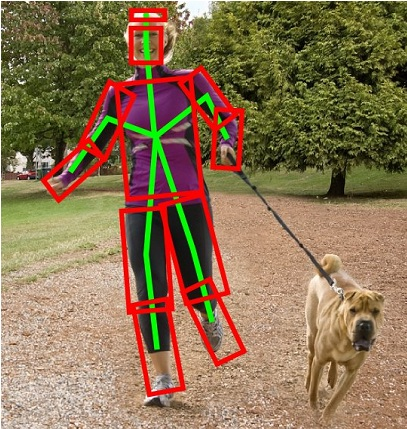
\includegraphics[width=.45\textwidth]{img/graph1.jpg}
    }
    \subfigure[概率图模型表示的图画式结构]{
        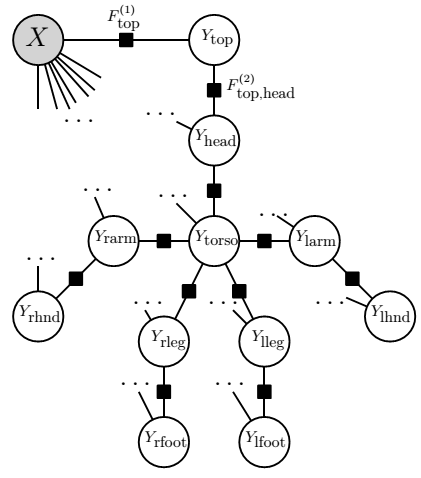
\includegraphics[width=.45\textwidth]{img/graph2.jpg}
    }
    \bicaption{概率图模型}{概率图模型}{Fig}{Graphic Model}
    \label{fig:graphmodel}
\end{figure}


\section{图画式结构}
基于对象的图画式结构模型是由部位的集合构成的,并且包含了部位之间的联系,像一个弹簧结构一样,有些部位之间有关联。
图画式结构模型采用形状特性来描述每个部位,用形变信息来描述相关联的两个部位。
本质上来说,它是一个很通用的模型,因为这个模型和具体描述每个部位的形状特征是无关的,研究者可以使用任意一种形状特征,比如方向梯度直方图(HOG)等,
而且这个模型和描述相关联部位的形变特征也是无关的,研究者也可以使用任意一种形变特征。
一般来讲,表示图画式结构模型的最自然的方式是无向图$G=(V, E)$,其中顶点集合为$V = \left\{v_1, v_2, \cdots, v_n \right\}$,对应了n个部位,
任意一条边$(v_i, v_j) \in E$ 代表了两个相关联顶点$v_i$和$v_j$之间的关系。
对于物体的信息,我们用配置信息$L = (l_1, l_2, \cdots, l_n)$ 来描述,其中$l_i$代表部位$v_i$的位置。
一般情况下,我们的$L$只代表物体的位置,但是配置信息其实还可以代表更多的信息,它代表了每个部位的表示方式。
每个部位的位置信息可以简单的描述它在图像中的像素位置,但是更复杂的、更多的参数也是可能的。
举例来说,对于我们文章中提出的隐式衣服属性模型,每个部位的配置信息包括位置、大小、方向等信息。

\begin{figure}
\centering
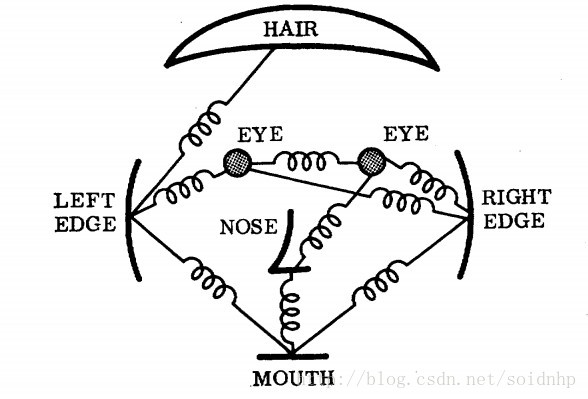
\includegraphics[width=0.9\textwidth]{img/ps.jpg}
\bicaption{人脸部弹簧模型}{人脸部弹簧模型}{Fig}{Pictorial Structure for Face Detection}
\label{fig:ps}
\end{figure}

在图画式结构模型的经典论文\cite{ps1}中,我们用能量函数来描述一个图画式结构模型和测试图片之间的不匹配程度,
而问题就是要最小化这个能量函数。
对于每一种所有部位的配置形式的损失或者能量,它与下面两方面内容有关系:
一是每个部位跟测试图片中这个位置的不匹配程度,而是两个部位的位置关系和形变模型的不匹配程度。
给定一张图片,用函数$m_i(l_i)$来测量部位$v_i$和测试图片中位置$l_i$的不匹配程度。
对于两个相关联的部位,我们用函数$d_{ij}(l_i, l_j)$来测量$(v_i, v_j)$和测试图片中位置$(l_i, l_j)$的不匹配程度。
因此,对于测试图片来说,和模型最匹配的配置信息形式应该是:

\begin{equation}
    \label{eq:pseq}
    L^{\*} = arg \min {\left( \sum_{i=1}^{n} m_i(l_i) + \sum_{ (v_i, v_j) \in E } d_{ij}(l_i, l_j) \right)}
\end{equation}

公式表示了一种最优的配置信息,它最小化了每个部位的不匹配程度$m_i$与每两个关联部位不匹配程度$d_{ij}$的和。
一般地,描述形变特征不匹配程度的函数往往只跟两个部位的相对位置有关系,这样使得模型可以很好的使用全局变换。
需要注意的是,一个图画式结构模型和测试图片的能量函数不只是跟每个单独部位的位置有关系,
而是依赖于所有的部位形状特征匹配度和所有相关联部位的形变特征匹配度的。

\begin{figure}[tbp]
    \centering
    \subfigure[]{
        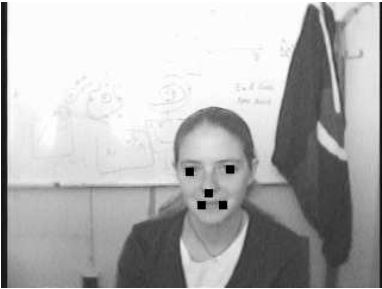
\includegraphics[width=.45\textwidth]{img/ps1.JPG}
    }
    \subfigure[]{
        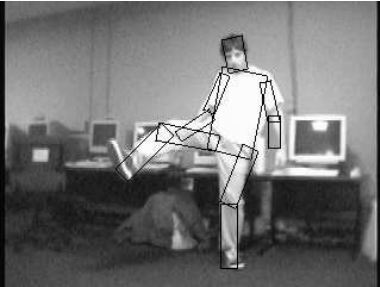
\includegraphics[width=.45\textwidth]{img/ps2.JPG}
    }
    \bicaption{用图画式结构检测出的一个简单的例子,人脸(a)和一个人体(b)。每张图片展示了需要检测的物体的全局最优解,
        这是算法检测出的结果。这个物体模型是从训练数据学习出来的。}{用图画式结构检测出的一个简单的例子,人脸(a)和一个人体(b)。每张图片展示了需要检测的物体的全局最优解,
        这是算法检测出的结果。这个物体模型是从训练数据学习出来的。}{Fig}{Sample results for detection of a face (a); and a human body (b). Each
image shows the globally best location for the corresponding object, as computed by
our algorithms. The object models were learned from training examples.}
    \label{fig:ps2}
\end{figure}


可以看出这个能量函数\ref{eq:pseq}是简单并且直观的。
然而前人的很多工作都是采用启发式的或者局部搜索技术,他们很难找出一个最优解,因为最优解的获得严重依赖于初始化的方式,初始化参数设置的好,那么就有可能获得最优解,否则会很被动。
而图画式结构模型提供了一种高效并且简单的方式,可以找到一个全局的最优解,并且不需要任何初始化步骤。

图画式结构模型不仅可以表示计算机视觉中图片中的人物躯干、脸部器官等,还可以表示更一般的物体。
例如,对于每个部位的外观模型,可以是颜色或者方向特征,或者是局部方向过滤器的响应等,
两个部位之间的关联也可以用更一般的形式来建模,比如“接近”,“在左边”,“在上方”,或者更精确的几何上的约束(比如联合角度)。
因为每个部位的外观模型和任意两个相连部位之间的形变模型都可以一般化,所以图画式结构模型提供了一个强大的框架。
假设我们想对人体躯干的外观特征进行建模,很自然地我们要将人体躯干建模为一系列有关节的部位,并且连接了不同的人体部位。
通过图画式结构模型,我们可以采用一个粗粒度的模型,用数目比较少的部位表示。
简单的部位外观模型和相连部位的形变模型的结合提供了足够的上下文信息来找到人体躯干,但是对于找出更一般的人体部位还是很困难的,还是一个很大的挑战,
比如“小腿”或“上臂”等。

\section{结构式学习}
在计算机视觉领域,从大数据中学习出来的强大的统计模型正在不断的改进。
这些模型都包含了一个丰富的内部结构,来反映真实问题中任务相关的变量之间的关系和约束。
本节主要介绍下一些在计算机视觉领域非常流行的结构化模型,更为精确的是基于离散变量的无向图模型,它可以表示一大类算法描述,
比如概率预测和最大化后验概率。
下面我们主要来看一下结构式学习在计算机视觉领域的应用。


一般来讲,计算机视觉的目的就是让计算机能够从图片数据中理解出更高层的语义信息。
这些图片数据可能来自于各种种类的格式或者形式,它可以是一张自然图片,也可以是多张卫星图片序列,沿着时间序列拍摄的。
同样地,我们所讲的高层次信息也是多种多样的,从像素级别的图片表面信息,到图片中一般的物体(比如车、动物等)级别的信息。

\begin{figure}
\centering
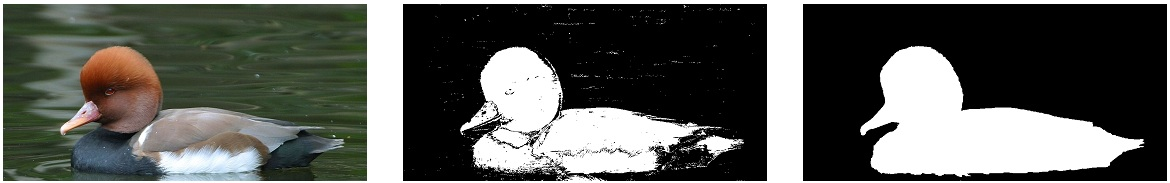
\includegraphics[width=0.9\textwidth]{img/struct.jpg}
\bicaption{首先第二幅图是利用简单的前背景和后背景分类器就可以输出,
而第三幅图必须使用像素之间的关联才可以做到图像分割。}{首先第二幅图是利用简单的前背景和后背景分类器就可以输出,
而第三幅图必须使用像素之间的关联才可以做到图像分割。}{Fig}{Pixel-wise separate classification by pixel only: 
noisy, locally inconsistent decisions. Joint optimum result with spatially consistent decisions.}
\label{fig:struct}
\end{figure}

上述所讲的任务一般会构建一个模型,这个模型是跟图像数据和高层次信息都有关的一个模型。
这个模型中包含了一组变量的集合,其中包括可观测的用来描述图片数据的变量,描述高层次信息的输出变量,
还有一类辅助变量,用来描述输入输出之间的关系等。
在这些变量之外,模型还定义了变量之间是怎么互相关联的,如何互相依赖的等。
这些变量和变量之间的关系构成了这个模型的结构。
结构化模型允许我们构建任意多的变量和变量之间的关联信息,从而可见结构化模型的表征能力是极其强大的,它可以表达出非常复杂的关系,
图像数据和任意感兴趣的高层次信息之间的关系,都可以用结构化模型来表征。

不止于构建一个单一的固定模型,我们还可以增加参数来描述变量之间的关系。
给定标记好的数据和已知的输出变量类型,我们可以调整模型的参数,从而学出一组使得观测变量和输出变量最匹配的参数。这即就是参数学习或模型训练。

\begin{figure}
\centering
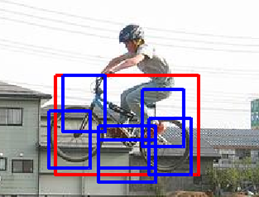
\includegraphics[width=0.7\textwidth]{img/dpm1.png}
\bicaption{自行车的检测案例}{自行车的检测案例}{Fig}{Example for bicycle detection.}
\label{fig:dpm1}
\end{figure}

\section{形变部位模型}
形变部位模型\cite{llsvm}DPM(Deformable Part Model)是一个非常成功的目标检测算法,
连续获得VOC(Visual Object Class)07,08,09年的检测冠军。
目前已成为众多分类器、分割、人体姿态和行为分类的重要部分。
2010年Pedro Felzenszwalb被VOC授予“终身成就奖”。
DPM可以看作是HOG(Histograms of Oriented Gradients)的扩展,大体思路与HOG一致。
先计算梯度方向直方图,然后用SVM(Support Vector Machine)训练得到物体的梯度模型(Model)。
有了这样的模板就可以直接用来分类了,简单理解就是模型和目标匹配。DPM只是在模型上做了很多改进工作。

\begin{figure}
\centering
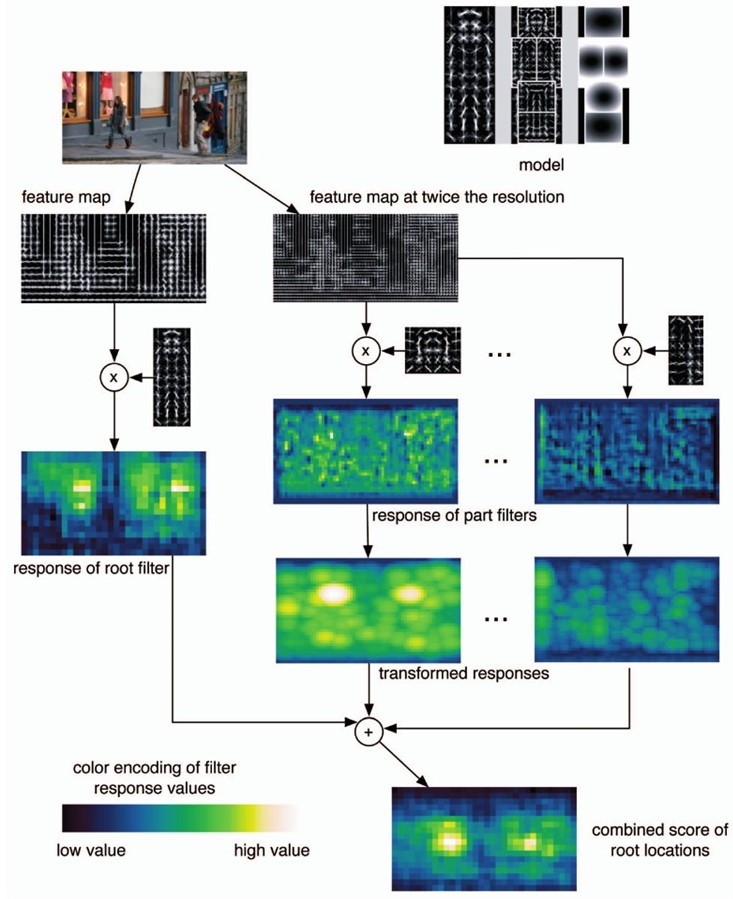
\includegraphics[width=0.9\textwidth]{img/dpm.jpg}
\bicaption{DPM模型的框架流程图}{DPM模型的框架流程图}{Fig}{The framework for DPM model}
\label{fig:dpm}
\end{figure}

上图是HOG论文中训练出来的人体模型。它是但模型,对直立的正面和背面人检测效果很好,较以前取得了重大的突破。
也是目前为止最好的特征(最近被CVPR2013年的一篇论文\cite{hsc}超过了)。
但是,如果是侧面呢,所以自然我们会想到利用更多的模型去构建。
DPM就使用了2个模型,主页上最新版本的程序使用了12个模型。
有了多模型,就可以解决视角的问题了,还有一个严重的问题,动物是动的,就算是没有生命的车也有很多款式,
单单有一个模型,如果动物动一下,人物运动一下,那模型就跟这个人的匹配程度就低了很多。
也就是说,我们的模型适应能力太差了,不能适应物体的运动,特别是非刚性物体的运动,自然我们又能想到添加子模型,比如给手一个子模型,
当手移动时,子模型能够检测到手的位置。把子模型和主模型的匹配程度综合起来,最简单的就是相加,那模型匹配程度就会提高。
还有我们要加入子模型和主模型中位置的偏移程度的损失,也就是综合得分要减去偏移的损失。
本质上就是要使用子模型和主模型的空间先验知识。



\section{本章小结}
本章介绍了与我们工作相关的一些背景知识,包括图模型、图画式结构模型、结构式学习、形变部位模型等。
图模型是我们算法的基础,它定义了一个非常强大的语言,将我们实际问题中变量的关系表示的非常清楚,
它表征了变量之间的概率关系,特别适合复杂问题的变量关系表示。
图画式结构模型提供了一个弹簧结构问题的优化算法,基于图模型将变量之间的关系通过一种特殊的结构构建起来,
特别适用于人体结构预测、人脸特征部位预测等实际问题。
结构式学习是很多机器学习问题的基础,它可以解决很多复杂问题,
包括自然语言处理中的问题,计算机视觉中的问题,语音识别中的问题等。
形变部位模型是近年来物体识别领域最火的一个模型,它为本文的工作提供了一个基础的想法框架。
通过对这些模型的介绍,使得对我们工作的背景和动机有一个清晰明确的认识,并且有助于对人体姿势预测整个领域有一个深入的了解,
并且有助于理解我们在本文中提出的模型算法。
